\documentclass[12pt]{beamer}
\newenvironment{ConCodigo}[1]
  {\begin{frame}[fragile,environment=ConCodigo]{#1}}
  {\end{frame}}
\graphicspath{{Imagenes/}{../Imagenes/}}
\usepackage[utf8]{inputenc}
\usepackage[spanish]{babel}
\usepackage{hyperref}
\usepackage{etex}
\reserveinserts{28}
\usepackage{amsmath}
\usepackage{amsthm}
\usepackage{mathtools}
\usepackage{multicol}
\usepackage{multirow}
\usepackage{tabulary}
%\usepackage{tabularx}
\usepackage{booktabs}
\usepackage{nccmath}
\usepackage{biblatex}
\usepackage{epstopdf}
\usepackage{graphicx}
\usepackage{siunitx}
\sisetup{scientific-notation=true}
%\usepackage{fontspec}
\usepackage{lmodern}
\usepackage{float}
\usepackage[format=hang, font=footnotesize, labelformat=parens]{caption}
\usepackage[autostyle,spanish=mexican]{csquotes}
\usepackage{standalone}
\usepackage{tikz}
\usepackage[siunitx]{circuitikz}
\usetikzlibrary{arrows,patterns,shapes}
\usetikzlibrary{decorations.markings}
\usetikzlibrary{arrows}
\usepackage{color}
%\usepackage{beton}
%\usepackage{euler}
%\usepackage[T1]{fontenc}
\usepackage[sfdefault]{roboto}  %% Option 'sfdefault' only if the base font of the document is to be sans serif
\usepackage[T1]{fontenc}
\renewcommand*\familydefault{\sfdefault}
\DeclareGraphicsExtensions{.pdf,.png,.jpg}
\usepackage{hyperref}
\renewcommand {\arraystretch}{1.5}
\newcommand{\python}{\texttt{python}}
\usefonttheme[onlymath]{serif}
\setbeamertemplate{navigation symbols}{}
\usetikzlibrary{patterns}
\usetikzlibrary{decorations.markings}
\tikzstyle{every picture}+=[remember picture,baseline]
%\tikzstyle{every node}+=[inner sep=0pt,anchor=base,
%minimum width=2.2cm,align=center,text depth=.15ex,outer sep=1.5pt]
%\tikzstyle{every path}+=[thick, rounded corners]
\setbeamertemplate{caption}[numbered]
\newcommand{\ptm}{\fontfamily{ptm}\selectfont}
%Se usa la plantilla Warsaw modificada con spruce
\mode<presentation>
{
  \usetheme{Warsaw}
  \setbeamertemplate{headline}{}
  \useoutertheme{default}
  \usecolortheme{beaver}
  \setbeamercovered{invisible}
}
\AtBeginSection[]
{
\begin{frame}<beamer>{Contenido}
\normalfont\mdseries
\tableofcontents[currentsection]
\end{frame}
}

\usepackage{listings}
\lstset{ %
language=Python,                % choose the language of the code
basicstyle=\small,       % the size of the fonts that are used for the code
numbers=left,                   % where to put the line-numbers
numberstyle=\small,      % the size of the fonts that are used for the line-numbers
stepnumber=1,                   % the step between two line-numbers. If it is 1 each line will be numbered
numbersep=5pt,                  % how far the line-numbers are from the code
backgroundcolor=\color{white},  % choose the background color. You must add \usepackage{color}
showspaces=false,               % show spaces adding particular underscores
showstringspaces=false,         % underline spaces within strings
showtabs=false,                 % show tabs within strings adding particular underscores
frame=single,   		% adds a frame around the code
tabsize=2,  		% sets default tabsize to 2 spaces
captionpos=b,   		% sets the caption-position to bottom
breaklines=true,    	% sets automatic line breaking
breakatwhitespace=false,    % sets if automatic breaks should only happen at whitespace
escapeinside={\%},          % if you want to add a comment within your code
stringstyle =\color{magenta},
keywordstyle = \color{blue},
commentstyle = \color{green},
identifierstyle = \color{red}
}
%\usepackage{siunitx}
%\usepackage[american,cuteinductors,smartlabels]{circuitikz}
%\usetikzlibrary{calc}
\title{Ecuaciones diferenciales ordinarias 4}
\subtitle{Curso de Física Computacional}
\author[]{M. en C. Gustavo Contreras Mayén}
%\email{curso.fisica.comp@gmail.com}
%\ptsize{10}
\begin{document}
\maketitle
\fontsize{14}{14}\selectfont
\spanishdecimal{.}
\begin{frame}{Contenido}
\tableofcontents[pausesections]
\end{frame}
\section{Estabilidad y rigidez.}
\begin{frame}
Hablando de manera general, un método de integración se dice que es estable si los efectos de errores locales, no se acumulan progresivamente, es decir, si el error global permanece acotado.
\\
\medskip
Si el método es inestable, si el error global se incrementa de manera exponencial, generando eventualmente un desbordamiento (overflow). La estabilidad no tiene nada que ver con la precisión, de hecho, un método impreciso puede ser muy estable.
\end{frame}
\begin{frame}
\frametitle{Determinantes de la estabilidad}
La estabilidad está determinada por tres factores:
\begin{enumerate}[<+->]
\item Las ecuaciones diferenciales.
\item El método de solución.
\item El valor del incremento $h$.
\end{enumerate}
Desafortunadamente, no es fácil determinar de antemano la estabilidad, a menos que la ecuación diferencial sea lineal.
\end{frame}
\subsection{Estabilidad del método de Euler}
\begin{frame}
\frametitle{Estabilidad del método de Euler}
Con el fin de ilustar la estabilidad, consideremos el problema lineal
\[y' = - \lambda y \hspace{2cm} y(0) = \beta \]
donde $\lambda$ es una constante positiva.
\\
\medskip
La solución exacta de este problema es
\[ y(x) = \beta e^{- \lambda x} \] 
\end{frame}
\begin{frame}
Veamos qué pasa cuando intentamos resolver numéricamente esta ecuación con el método de Euler.
\[ y(x+h) = y(x) + h y'(x) \]
sustituimos $y'(x) = - \lambda y(x)$, para obtener
\[ y(x+h) = (1-\lambda h) y(x) \]
Si $\vert 1- \lambda h \vert > 1$, se nota claramente que el método es inestable ya que el valor de $\vert y \vert$ se incrementa en cada paso de integración.
\\
\medskip
Por tanto, el método de Euler es estable solamente si $\vert 1- \lambda h \vert \leq 1$, o
\[ h \leq \dfrac{2}{\lambda}\]
\end{frame}
\begin{frame}
Los resultados se pueden extender a un sistema de $n$ ecuaciones diferenciales de la forma
\[ \mathbf{y}' = - \mathbf{\Lambda y}\]
donde $\mathbf{\Lambda}$ es una matriz constante con valores propios positivos $\lambda_{i}$, con $i=1,2,\ldots,n$. Se puede demostrar que el método de integración de Euler es estable si
\[ h < \dfrac{2}{\lambda_{max}}\]
donde $\lambda_{max}$ es el valor propio mayor de $\mathbf{\Lambda}$.
\end{frame}
\section{Rigidez}
\begin{frame}
\frametitle{Rigidez}
Un problema de valores iniciales se dice que es \emph{rígido}, si algunos de los elementos del vector solución $\mathbf{y}(x)$ varían mucho más rápido con respecto a $x$, que otros.
\\
\medskip
La rigidez puede predecirse fácilmente del conjunto de ED $\mathbf{y}' = - \mathbf{\Lambda y}$ con una matriz de coeficientes constantes $\mathbf{\Lambda}$.
\end{frame}
\begin{frame}
La solución de esas ecuaciones es:
\[ \mathbf{y}(x) = \sum_{i} C_{i} \mathbf{v}_{i} \exp(-\lambda_{i} x)\]
donde $\lambda_{i}$ son los valores propios de $\mathbf{\Lambda}$ y $\mathbf{v}_{i}$ son los correspondientes vectores propios. Es evidente que el problema es rígido si hay una gran disparidad en las magnitudes de los valores propios positivos.
\end{frame}
\begin{frame}
La integración numérica de las ecuaciones rígidas requiere un cuidado especial. El tamaño del paso $h$ necesario para la estabilidad está determinado por el valor propio más grande ($\lambda_{max}$), aunque si los términos $\exp(-\lambda_{max} x)$ en la solución decaen muy rápidamente y se vuelven insignificantes a medida que nos alejamos del origen.
\end{frame}
\begin{frame}
Por ejemplo, sea la siguiente EDO
\[ y'' + 1001 y' + 1000 y = 0 \]
usando $y_{0} = y$ junto con $y_{1} = y_{1}$, el conjunto equivalente de 1-EDO, resulta
\[ \mathbf{y}' = \begin{bmatrix}
y_{1} \\
-1000 y_{0} - 10001 y_{1}
\end{bmatrix} \]
En este caso
\[ \mathbf{\Lambda} = \begin{bmatrix}
0 & -1 \\
1000 & 1001 
\end{bmatrix}\]
\end{frame}
\begin{frame}
Los valores propios (\emph{eigenvalues}) son las raíces de:
\[ \vert \mathbf{\Lambda} - \lambda \mathbf{I} \vert = \begin{vmatrix}
- \lambda & -1 \\
1000 & 1001-\lambda
 \end{vmatrix} = 0\]
expandiendo el determinante, tenemos que
\[ - \lambda (1001 - \lambda) + 1000 = 0 \]
las soluciones son $\lambda_{1} = 1$ y $\lambda_{2} = 1000$
Claramente la ecuación es rígida; se necesita que $h < 2/\lambda_{2} = 0.002$ para que el método de Euler sea estable.
\\
\medskip
El método de Runge-Kutta tendría aproximadamente la misma limitación en el tamaño del paso.
\end{frame}
\begin{frame}
\frametitle{Ejemplo}
Mostrar que el problema
\[ y'' = - \dfrac{19}{4}y - 10 y', \hspace{1cm} y(0)=-9, \hspace{1cm} y'(0)=0 \]
\begin{enumerate}
\item Es ''moderadamente'' rígido.
\item Estimar el valor de $h_{max}$, el valor mayor de $h$ con el cual el método RK es estable. \item Revisa al calcular $y(10)$ con $h \simeq h_{max}/2$ y $h \simeq 2 h_{max}$.
\end{enumerate}
\end{frame}
\begin{frame}
\frametitle{Solución Punto 1}
Con la notación que ya manejamos, hacemos $y=y_{0}$ y $y'=y_{1}$, para nuestro sistema de EDO-1
\[ \mathbf{y}' = \begin{bmatrix}
y_{1} \\
- \dfrac{19}{4} y_{0} - 10 y_{1}
\end{bmatrix}  =
- \mathbf{\Lambda}
\begin{bmatrix}
y_{0} \\
y_{1}
\end{bmatrix}
\]
\pause
donde
\[ \mathbf{\Lambda} = 
\begin{bmatrix}
0 & -1 \\
\dfrac{19}{4} & 10
\end{bmatrix}
\]
\end{frame}
\begin{frame}
Los valores propios de $\mathbf{\Lambda}$ están dados por
\[ \vert \mathbf{\Lambda} - \lambda \mathbf{I} \vert = 
\begin{vmatrix}
- \lambda & -1 \\
\dfrac{19}{4} & 10 - \lambda
\end{vmatrix} = 0 \]
Que nos devuelve $\lambda_{1} = 1/2$ y $\lambda_{2} = 19/2$.
\\
\medskip
Como $\lambda_{2}$ es un poco más grande que $\lambda_{1}$, las ecuaciones son ''moderadamente'' rígidas.
\end{frame}
\begin{frame}
\frametitle{Solución Punto 2}
Un estimado para el límite superior de $h$ en donde es estable el método se puede obtener de la expresión indicada anteriormente
\[ h_{max} = \dfrac{2}{\lambda_{max}} = \dfrac{2}{19/2} = 0.2153\]
Aunque esta fórmula es válida estrictamente para el método de Euler, por lo general se puede utilizar para las fórmulas de integración de orden superior.
\end{frame}
\begin{frame}
\frametitle{Solución Punto 3}
Haciendo $h_{1} = \lambda_{max}/2 = 0.10765 \simeq 0.1$ y ejecutando el código, tenemos que
\begin{tabular}{c | c | c}
$x$ & $y[0]$ & $y[1]$ \\ \hline
$0.0000e+000$ & $-9.0000e+000$ & $0.0000e+000$ \\ \hline
$1.0000e+001$ & $-6.4011e-002$ & $3.2005e-002$ \\ \hline
\end{tabular}
\\
\medskip
La solución analítica del problema es:
\[ y(x) = -\dfrac{19}{2} \exp \left( - \frac{x}{2} \right) + \dfrac{1}{2} \exp \left(- \frac{19x}{2} \right) \]
evaluando $y(10)= 0.064011$, que es el valor que se obtiene con el método RK4.
\end{frame}
\begin{frame}
Ahora haciendo $h_{2} = 2 \lambda_{max} = 0.4306$ y ejecutando nuevamente el código, tenemos que
\begin{tabular}{c | c | c}
$x$ & $y[0]$ & $y[1]$ \\ \hline
$0.0000e+00$ & $-9.0000e+00$ & $0.0000e+00$ \\ \hline
$1.0000e+01$ & $1.9244e+16$ & $-1.8282e+17$ \\ \hline
\end{tabular}
\\
\medskip
En donde vemos que la inestabilidad del método se hace evidente por el valor de $h$.
\end{frame}
\section{Métodos multipaso}
\begin{frame}
\frametitle{Métodos multipaso}
La determinación del tamaño de $h$ adecuad, puede ser un dolor de cabeza en los procedimientos de integración numérica: si es demasiado grande, el error de truncamiento resulta ser inaceptable; si su demasiado pequeño, estamos desperdiciando recursos computacionales.
\\
\medskip
Por otra parte, un tamaño de paso constante puede no ser adecuado para toda la gama de integración. Por ejemplo, si la curva solución comienza con cambios rápidos antes de convertirse en suave (como en un problema de rigidez), debemos utilizar una $h$ pequeña al principio y aumentarla cuando llegamos a la zona lisa.
\end{frame}
\begin{frame}
Aquí es donde los métodos adaptativos llegan para apoyarnos: estiman el error de truncamiento en cada paso de integración y ajustan automáticamente el tamaño de paso para mantener el error dentro de los límites prescritos.
\end{frame}
\begin{frame}
Los métodos de Runge-Kutta adaptativos utilizan las denominadas fórmulas de integración incorporadas.
\\
\medskip
Estas fórmulas vienen en pares: una fórmula tiene el orden de integración $m$, la otra es de orden $m + 1$. La idea es utilizar ambas fórmulas para avanzar en la solución de $x$ a $x + h$.
\\
\medskip
De los resultados $\mathbf{y}_{m}(x+h)$ y $\mathbf{y}_{m+1}(x+h)$ podemos estimar el error de truncamiento en la fórmula de orden $m$
\[ \mathbf{E}(h) = \mathbf{y}_{m+1}(x+h) - \mathbf{y}_{m}(x+h) \]
Lo que hace atractivo el uso de fórmulas embebidas, ya que comparten puntos donde $\mathbf{F}(x,\mathbf{y})$ son evaluados.
\end{frame}
\begin{frame}
Esto significa que cada $\mathbf{y}_{m}(x+h)$ ha sido calculado, se requiere un esfuerzo pequeño para calcular $\mathbf{y}_{m+1}(x+h)$
\end{frame}
\begin{frame}
\frametitle{Fórmulas Runge-Kutta-Fehlberg}
Se presentan las fórmulas incoporadas de orden 5 y 4 obtenidas por Erwin Fehlberg, por lo que se conocen como las fórmulas Runge-Kutta-Felhlberg (RKF45)
\begin{eqnarray*}
\mathbf{K}_{0} &=& h \mathbf{F}(x,y) \\
\mathbf{K}_{i} &=& h \mathbf{F} \left( x  + A_{i} h, \mathbf{y} + \sum_{j=0}^{i-1} B_{ij}\mathbf{K}_{j} \right) \\
\mathbf{y}_{5}(x+h) &=& \mathbf{y}(x) + \sum_{i=0}^{5} C_{i} \mathbf{K}_{i} \hspace{0.5cm} \mbox{fórmula de 5o. orden} \\
\mathbf{y}_{4}(x+h) &=& \mathbf{y}(x) + \sum_{i=0}^{5} D_{i} \mathbf{K}_{i} \hspace{0.5cm} \mbox{fórmula de 4o. orden}
\end{eqnarray*}
\end{frame}
\begin{frame}
Los coeficientes que aparecen en las fórmulas no son únicos. En la siguiente tabla se muestran los valores de los coeficientes.
\begin{tabular}{| c | c | c c c c c | c | c |}
\hline
$i$ & $A_{i}$ & & & $B_{ij}$ & & & $C_{i}$ & $D_{i}$ \\ \hline
$0$ & - & - & - & - & - & - &  $\frac{37}{378}$ & $\frac{2825}{27648}$ \\ \hline
$1$ & $\frac{1}{5}$ & $\frac{1}{5}$ & - & - & - & - &  $0$ & $0$ \\ \hline
$2$ & $\frac{3}{10}$ & $\frac{3}{40}$ & $\frac{9}{40}$ & - & - & - &  $\frac{250}{621}$ & $\frac{18575}{48384}$ \\ \hline
$3$ & $\frac{3}{5}$ & $\frac{3}{10}$ & $-\frac{9}{10}$ & $\frac{6}{5}$ & - & - &  $\frac{125}{594}$ & $\frac{13525}{55296}$ \\ \hline
$4$ & $1$ & $-\frac{11}{54}$ & $\frac{5}{2}$ & $-\frac{70}{27}$ & $\frac{35}{27}$ & - &  $0$ & $\frac{277}{14336}$ \\ \hline
$5$ & $\frac{7}{8}$ & $\frac{1631}{55296}$ & $\frac{175}{512}$ & $\frac{575}{13824}$ & $\frac{44275}{4096}$ & $\frac{253}{4096}$ &  $\frac{512}{1771}$ & $\frac{1}{4}$ \\ \hline
\end{tabular}
\end{frame}
\begin{frame}
\frametitle{Ejemplo}
La fuerza de arrastre aerodinámico en un objeto en caída libre se puede aproximar por
\[ F_{D} = av^{2} \exp(-by) \]
donde
\begin{itemize}
\item $v$ es la velocidad del objeto en m/s
\item $y$ es la elevación del objeto en metros.
\item $a=7.45$ kg/m
\item $b= 10.53 \times 10^{-5} \hspace{0.1cm} \mbox{m}^{-1}$
\end{itemize}
\end{frame}
\begin{frame}
El término exponencial representa el cambio de densidad del aire con la elevación. La ecuación diferencial que describe la caída del objeto es
\[ m \ddot{y} = -mg + F_{D} \]
donde $g=9.80665 \hspace{0.1cm} \mbox{m/s}^{2}$ y $m=114 \hspace{0.1cm} \mbox{kg}$ es la masa del objeto. Si el objeto se libera de una altura de $9$ km, calcula su altura y velocidad luego de $10$ segundos de caída, utiliza el método RK adaptativo.
\end{frame}
\begin{frame}
\frametitle{Solución}
La ecuación diferencial y las condiciones de frontera son
\[ \begin{split}
\ddot{y} &= - g + \dfrac{a}{m} \dot{y}^{2} \exp(-by) \\
&= -9.80665 + \dfrac{7.45}{114} \dot{y}^{2} \exp(-10.53 \times 10^{-5}y) \\
{} \\
&{} y(0) = 9000 m \hspace{1cm} \dot{y}(0)=0
\end{split} \]
\end{frame}
\begin{frame}
Haciendo $y_{0}= y$ y $y_{1}=\dot{y}$, obtenemos el sistema de EDO-1
\fontsize{12}{12}\selectfont
\[ \begin{split}
\mathbf{\dot{y}} &= \begin{bmatrix}
\dot{y}_{0} \\
\dot{y}_{1}
\end{bmatrix} \\
&= \begin{bmatrix}
y_{1} \\
-9.80665 + (65.351 \times 10^{-3} y_{1}^{2} \exp(-10.53 \times 10^{-5} y_{0}
\end{bmatrix}
\end{split} \]
\[ \mathbf{y}(0) = 
\begin{bmatrix}
9000 \mbox{ m} \\
0
\end{bmatrix} \]
\end{frame}
\begin{frame}
\frametitle{Solución}
\begin{tabular}{c | c | c}
$x$ & $y[0]$ & $y[1]$ \\ \hline
$0.0000e+00$ & $9.0000e+03$ & $0.0000e+00$ \\ \hline
$5.0000e-01$ & $8.9988e+03$ & $-4.8043e+00$ \\ \hline
$2.0584e+00$ & $8.9821e+03$ & $-1.5186e+01$ \\ \hline
$3.4602e+00$ & $8.9581e+03$ & $-1.8439e+01$ \\ \hline
$4.8756e+00$ & $8.9312e+03$ & $-1.9322e+01$ \\ \hline
$6.5347e+00$ & $8.8989e+03$ & $-1.9533e+01$ \\ \hline
$8.6276e+00$ & $8.8580e+03$ & $-1.9541e+01$ \\ \hline
$1.0000e+01$ & $8.8312e+03$ & $-1.9519e+01$ \\ \hline
\end{tabular}
\end{frame}
\begin{frame}
Nótese que el primer paso que se realizó, se hizo con el valor de $h=0.5$, aparentemente el error fue bueno sin que la tolerancia fuera rebasada, por lo tanto se aceptó este valor.
\\
\medskip
Los pasos posteriores, que se calcuan de acuerdo a lo visto anteriormente, son considerablemente mayores.
\\
\medskip
Para el $t=10$ el objeto se mueve con una velocidad $v=-\dot{y}=19.52 \mbox{ m/s}$ y se encuentra a una altura de $8831 \mbox{ m}$.
\end{frame}
\begin{frame}
\frametitle{Otro ejemplo (ya trabajado anteriormente)}
Integrar el problema ''moderamente'' rígido
\[ y'' = -\dfrac{19}{4} y - 10 y' \hspace{1cm} y(0)=-9, \hspace{0.3cm} y'(0)=0 \]
de $0$ a $10$ con el método RK adaptativo y gráfica los resultados.
\end{frame}
\begin{frame}
\frametitle{Solución}
\begin{figure}
	\centering
	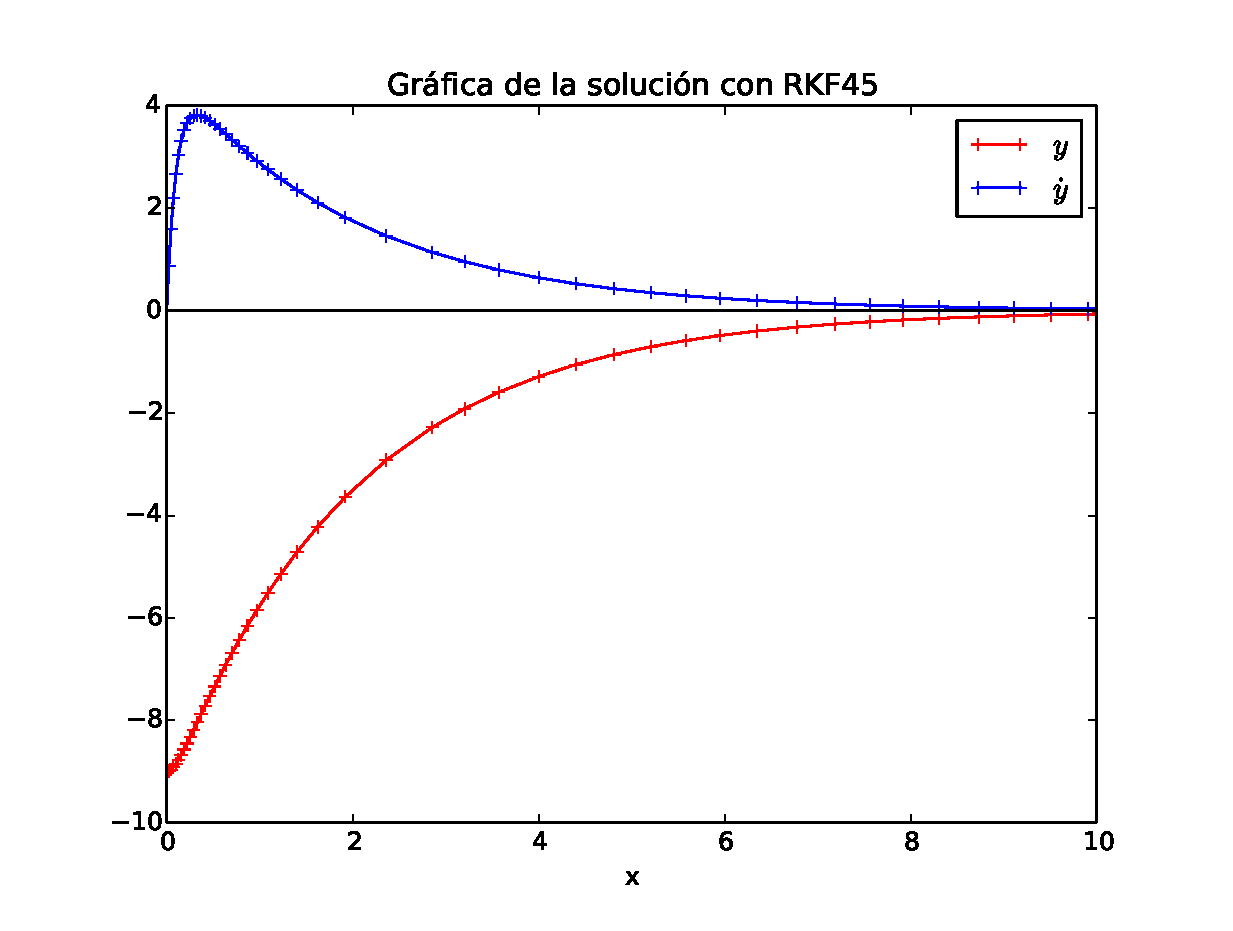
\includegraphics[scale=0.5]{Imagenes/MetodoRKF45.eps} 
\end{figure}
\end{frame}
\begin{frame}
Los resultados coinciden con la solución analítica. Las gráficas que se muestran $y$ y para $y'$ son del cuarto paso de integración.
\\
\medskip
Nótese elevada densidad de puntos cerca de $x=0$ donde $y'$ cambia muy rápido. Conforme la curva de $y'$ se suaviza, la distancia entre los puntos se incrementa.
\end{frame}
\section{EDO con valores en la frontera y valores propios}
\begin{frame}
\frametitle{Problemas con valores en la frontera y valores propios}
Otra tipo de problemas de la física requiere la solución de ecuaciones diferenciales con valores de las magnitudes físicas o sus derivadas en las fronteras de una región.
\\
\medskip
\pause
Por ejemplo:
\begin{itemize}
\item La solución de la ecuación de Poisson con una  distribución de carga dada y valores conocidos de potencial electrostático en la frontera.
\item La ecuación de Schrödinger estacionaria con un potencial dado y  
condiciones de frontera.
\end{itemize}
\end{frame}
\begin{frame}
Un problema de típico de valores en la frontera en física, por lo general se presenta en forma de una ecuación diferencial de segundo orden:
\begin{equation}
u'' = f(u, u';x)
\label{eq:ecuacion1}
\end{equation} 
donde $u$ es una función de $x$; $u'$ y $u''$ son las derivadas de primer y segundo orden de $u$ con respecto a $x$, $f(u,u';x)$ es una función de $u$, $u'$ y $x$. Tanto $u$ o $u'$ están dadas como puntos en la frontera.
\end{frame}
\begin{frame}
Considera que sin pérdida de generalidad, siempre podemos elegir un sistema coordenado tal que las fronteras del sistema sean $x=0$ y $x=1$, siempre y cuando el sistema sea finito.
\\
\medskip
Por ejemplo, para un problema dado si el sistema tiene las fronteras en $x=x_{1}$ y $x=x_{2}$, siempre podemos hacer $x'=0$ y $x'=1$ con una transformación
\begin{equation}
x' = \dfrac{x-x_{1}}{x_{2} - x_{1}}
\end{equation} 
\end{frame}
\begin{frame}
Para problemas de una dimensión, tenemos un total de cuatro tipo de condiciones de frontera:
\begin{enumerate}
\item $u(0) = u_{0}$ y $u(1) = u_{1}$ 
\item $u(0) = u_{0}$ y $u'(1) = v_{1}$
\item $u'(0) = v_{0}$ y $u(1) = u_{1}$
\item $u'(0) = v_{0}$ y $u'(1) = v_{1}$   
\end{enumerate}
\end{frame}
\begin{frame}
Un problema de valores en la frontera es más difícil de resolver que un problema de valores iniciales.
\\
\medskip
Si queremos resolver un problema de valores iniciales del tipo de la ecuación (\ref{eq:ecuacion1}), donde re-emplazamos $x$ por $t$ y las condiciones iniciales $u(0) = u_{0}$ y $u'(0) = v_{0}$, podemos transformar la ED en un conjunto de dos EDO-1, como lo hemos venido haciendo.
\\
\medskip
Sin embargo, para el problema de valores en la frontera (VEF), sólo conocemos $u(0)$ o $u'(0)$, que no es lo suficiente para utilizar alguno de los algoritmos que conocemos para las EDO-1 de valores iniciales (Taylor, Euler, RK4)
\end{frame}
\section{Problemas de valores propios}
\begin{frame}
\frametitle{Problemas de valores propios}
Los problemas típicos de valores propios son aún más complicados, ya que al menos un parámetro más, el \emph{valor propio}, está involucrado en la ecuación, por ejemplo:
\begin{equation}
u'' = f(u, u'; x; \lambda)
\label{eq:ecuacion_vp}
\end{equation}
junto con un conjunto de condiciones de frontera, definen un problema de valores propios.
\\
\medskip
El valor propio $\lambda$(también llamado \emph{eigenvalor}), puede tener sólo algunos valores determinados  con el fin de proporcionar soluciones aceptables de la ecuación, con las condiciones de frontera establecidas.
\end{frame}
\begin{frame}
\frametitle{Ejemplo}
Consideremos las vibraciones longitudinales a lo largo de una cuerda elástica, la ecuación que describe la solución estacionaria de las ondas elásticas es
\begin{equation}
u''(x) = - k^{2} u(x)
\end{equation}
donde $u(x)$ es el desplazamiento sobre el punto de equilibrio $x$ y los valores permitidos de $k^{2}$ son los valores propios del problema.
\\
\medskip
El vector de onda $k$ en la ecuación, está relacionado con la velocidad de fase $c$ de la onda a lo largo de la cuerda, y la frecuencia angular $\omega$ permitida, por la relación
\begin{equation}
\omega = ck
\end{equation}
\end{frame}
\begin{frame}
Si los extremos de la cuerda están fijos ($x=0$ y $x=1$), las condiciones de frontera son por tanto: $u(0)=u(1)=0$. Si un extremo de la cuerda ($x=0$) está fijo y el otro libre ($x=1$), las condiciones de frontera ahora son $u(0)=0$ y $u'(0)=1$. Para este problema, podemos obtener una solución analítica.
\\
\medskip
Por ejemplo, si los extremos de la cuerda están fijos, las funciones propias
\begin{equation}
u_{l}(x) = \sqrt{2} \sin k_{l} x
\end{equation}
son las posibles soluciones de la ED.
\\
\medskip
\pause
Los valores propios están dados por
\begin{equation}
k_{l}^{2} = (l \pi)^{2}
\end{equation}
con $l=1,2,\ldots,\infty$. 
\end{frame}
\begin{frame}
La solución completa de las ondas a lo largo de la cuerda elástica están dadas por una combinación lineal de las funciones propias con las soluciones de valores iniciales, en este caso
\begin{equation}
u(x,t) = \sum_{l=1}^{\infty} (a_{l} \sin \omega_{l} t + b_{i} \cos \omega_{l} t) u_{l}(x)
\end{equation}
donde $\omega_{l} = c k_{l}$, $a_{l}$ y $b_{l}$ son los coeficientes determinados por las condiciones iniciales.
\end{frame}
\section{Método de disparo}
\begin{frame}
\frametitle{Método de disparo}
Un método sencillo para resolver problemas de ED-CVF (ecuación \ref{eq:ecuacion1}) y los problemas de valores propios (ecuación \ref{eq:ecuacion_vp}), es el llamado \emph{método de disparo}.
\\
\medskip
Veamos cómo funciona para problemas CVF y luego, generalizar para problemas de valores propios.
\end{frame}
\begin{frame}
Como hemos hecho en el caso de tener un problema de una ED de orden 2, hacemos un cambio de variable, para dejar un sistema de EDO-1, haciendo $y_{1}=u$ y $y_{2}=u'$, por tanto
\begin{eqnarray}
\dfrac{dy_{1}}{dx} &=& y_{2} \\
\dfrac{dy_{2}}{dx} &=& f(y_{1}, y_{2}; x)
\end{eqnarray}
suponiendo las siguientes CVF $u(0)= u_{0}$ y $u(1)= u_{1}$. Para otro tipo de problemas con otras CVF, se pueden resolver de manera similar.
\end{frame}
\begin{frame}
El punto importante es hacer que el problema se parezca a un problema de valores iniciales, utilizando un parámetro que se ajuste, por lo que la solución se obtiene al variar el parámetro.
\\
\medskip
Como $u(0)$ ya está dado, podemos hacer una estimación para la derivada de primer orden en $x=0$, por ejemplo, $u'(0)=\alpha$. Donde $\alpha$ es el parámetro que estará variando.
\\
\medskip
\pause
Para un valor específico de $\alpha$, podemos integrar la ecuación para $x=1$ con alguna de las técnicas que hemos visto para EDO-1.
\end{frame}
\begin{frame}
Considerando que la elección inicial de  $\alpha$ difícilmente pudiese ser la derivada en $x = 0$, el valor de la función $u_{\alpha} (1)$, resultante de la integración con $u'(0) = \alpha$  para $x = 1$, podría no ser el mismo que $u_{1}$.
\\
\medskip
La idea del método de disparo es utilizar alguno de los algoritmos de búsqueda de la raíz para encontrar la $\alpha$ apropiada, que asegure $f(\alpha) = u_{\alpha} (1) - u_{1} = 0$, con una tolerancia $\delta$ dada.
\end{frame}
\begin{frame}
\frametitle{Ejemplo}
Hagamos un ejercicio para revisar el método. Sea la siguiente EDO-2
\begin{equation}
u'' = - \dfrac{\pi^{2}}{4}(u+1)
\end{equation}
y las CVF son $u(0)=0$ y $u(1)=1$. 
\\
\medskip
\pause
Definimos $y_{1}=u$ y $y_{2}=u'$, por lo que tenemos ahora
\begin{eqnarray}
\dfrac{dy_{1}}{dx} &=& y_{2} \\
\dfrac{dy_{2}}{dx} &=& - \dfrac{\pi^{2}}{4}(y_{1} + 1)
\end{eqnarray}
\end{frame}
\begin{frame}
Asumimos que la ecuación tiene los valores iniciales $y_{1}(0)=0$ y $y_{2}(0) = \alpha$.
\\
\medskip
\pause
El valor de $\alpha$ tendrá que ajustarse para que $f(\alpha) = u_{\alpha}(1) - 1 = 0$.
\\
\medskip
Podemos combinar el método de la secante y resolver el sistema de EDO-1 como lo hemos venido haciendo.
\\
\medskip
Resuelve y grafica el problema usando primero un valor de $\alpha=1.0$ y luego con $\alpha=4.0$. El problema cuenta para el Tema 3 y se considera resuelto cuando proporcionas el valor de $\alpha$ con el cual se cumplen las CVF y su respectiva gráfica.
\end{frame}
\begin{frame}[fragile]
\frametitle{Solución con $y0 = array([0.0,\alpha=1.0])$}
\begin{figure}
	\centering
	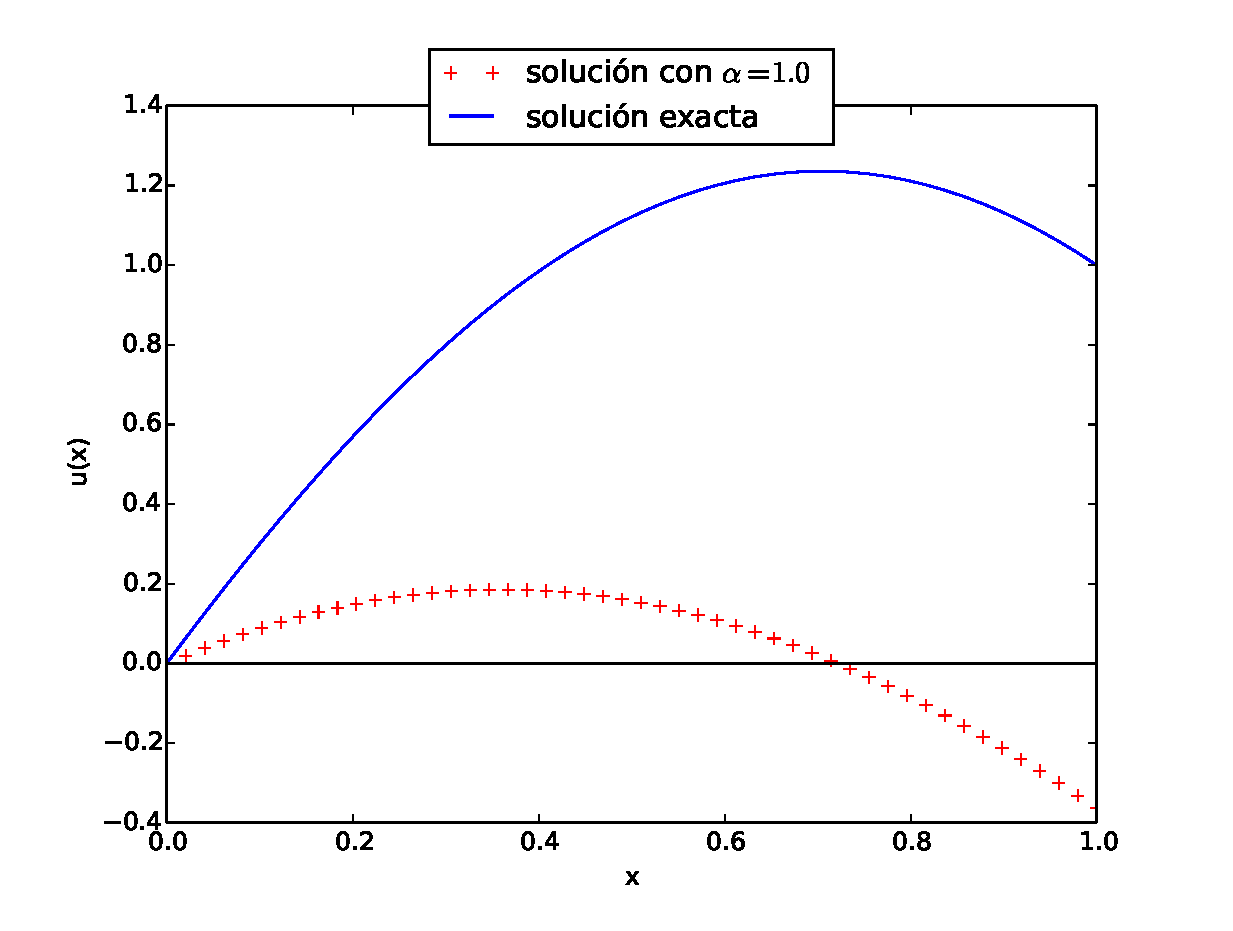
\includegraphics[scale=0.5]{MetodoDisparo2014_01.eps}
\end{figure}
\end{frame}
\begin{frame}[fragile]
\frametitle{Solución con $y0 = array([0.0,\alpha=4.0])$}
\begin{figure}
	\centering
	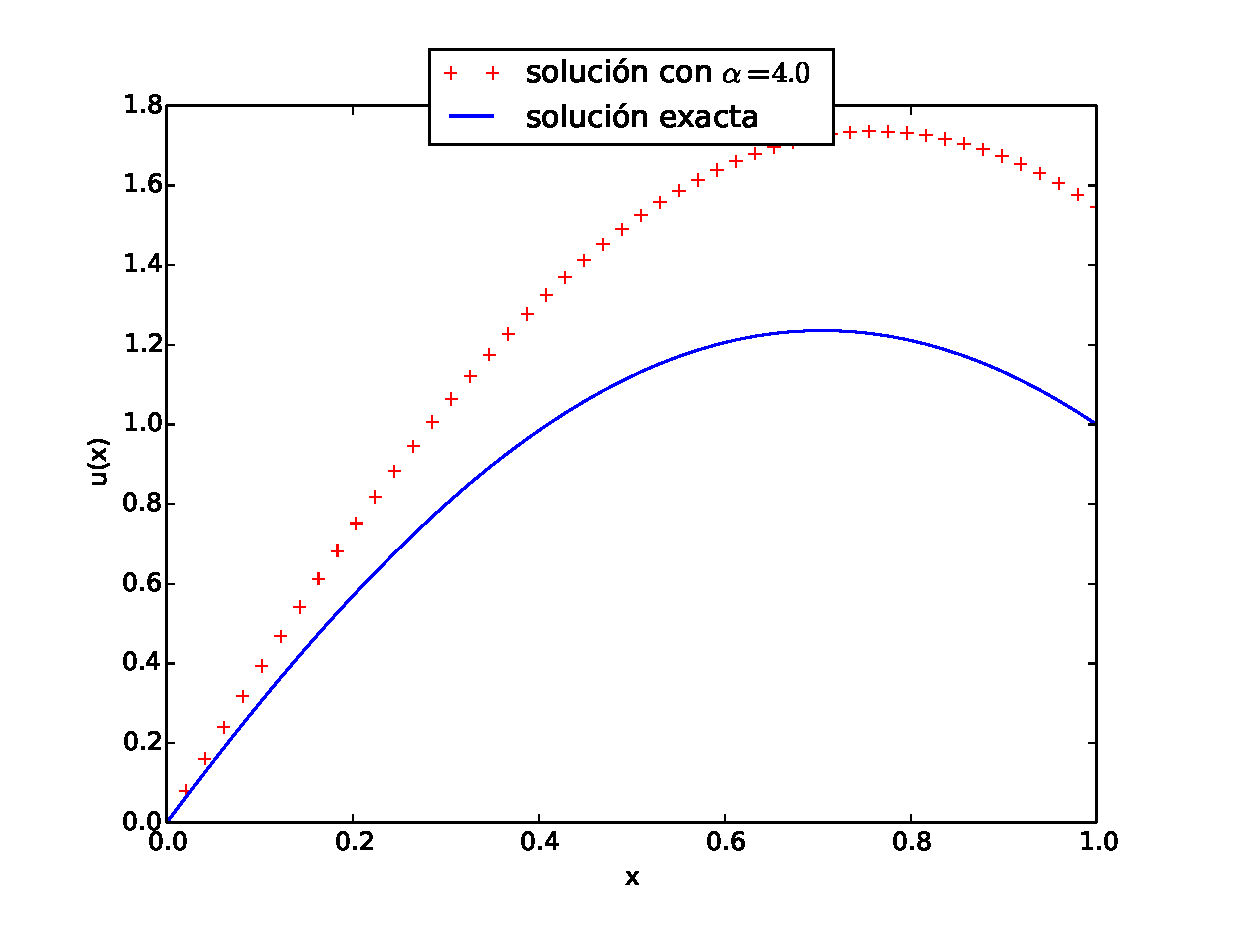
\includegraphics[scale=0.5]{MetodoDisparo2014_02.eps}
\end{figure}
\end{frame}
\begin{frame}
\frametitle{¿Qué hacemos?}
El siguiente paso es encontrar el valor de la raíz en donde $f(\alpha) = u_{\alpha}(1) - 1 = 0$.
\\
\medskip

Revisando los valores que obtenemos para $\alpha$:
\\
\medskip
$u_{1.0}(1) = -0.3633$ \\
$u_{4.0}(1) = 1.5464$
\\
\medskip
Por lo que necesariamente hay una raíz que debemos de utilizar para sustituirla en nuestro problema.
\end{frame}
\begin{frame}
El problema CVF se resuelve de manera exacta, la solución analítica es:
\begin{equation}
u(x) = \cos\left(\frac{x \pi}{2}\right) + 2 \sin \left(\frac{x \pi}{2}\right) -1
\end{equation}
\end{frame}
\begin{frame}
\frametitle{Pasos a realizar}
\begin{enumerate}
\item Construir una tabla de valores $\alpha$ y $f(\alpha) = u_{\alpha}(1) - 1$.
\item Usando el método de la secante, obtener el valor de la raíz tal que $f(\alpha)=0$. El método de la secante que construimos en el Tema 2, requiere de dos valores iniciales, para esa función, dabamos una función $f$ que python evalúa al momento, ahora nuestra función es una tabla de pares ordenados $\alpha$ y $f(\alpha)$, por lo que hay que ajustar nuestro código para que reciba esos valores y nos devuelva la raíz.
\item El valor de la raíz, lo usamos como argumento en $y0=[0.0, \alpha]$ y resolvemos la ecuación diferencial.
\end{enumerate}
\end{frame}
\begin{frame}[fragile]
\frametitle{Solución con $y0 = array([0.0,\alpha=??])$}
\begin{figure}
	\centering
	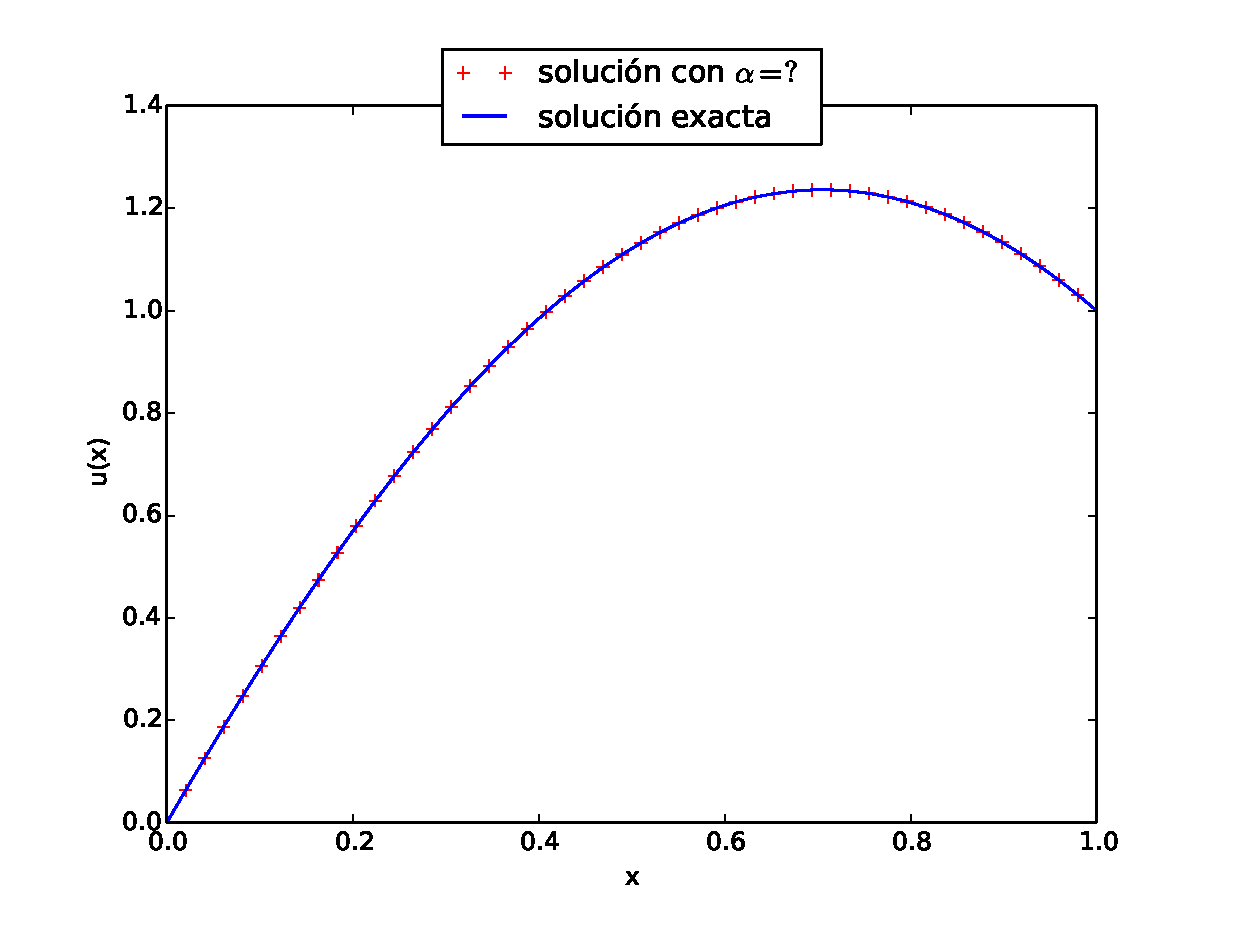
\includegraphics[scale=0.5]{MetodoDisparo2014_03.eps}
\end{figure}
\end{frame}
\begin{frame}
Problemas con otros tipos de CVF se pueden resolver de manera similar. Por ejemplo:
\\
\medskip
si $u'(0)=v_{0}$ y $u(1)=u_{1}$ están dados, podemos hacer una estimación de $u(0)=\alpha$ e integrar el conjunto de ecuaciones de $y_{1}$ y $y_{2}$ en $x=1$. La raíz a buscar está en $f(\alpha) = u_{\alpha}(1) - u_{1} = 0$. Aquí el valor de $u_{\alpha}(1)$ es el resultado de la ecuación con $u(0)=\alpha$.
\end{frame}
\begin{frame}
Cuando se aplica el método de disparo para los problemas de valores propios, el parámetro a ajustar no es mayor que el valor propio del problema.
\\
\medskip
Por ejemplo, si están dados $u(0)=u_{0}$ y $u(1)=u_{1}$, podemos integrar la ecuación con $u'(0)= \alpha$, que es un valor pequeño. Luego, buscamos la raíz de $f(\lambda) = u_{\lambda}(1) - u_{1}=0$ variando $\lambda$.
\\
\medskip
Cuando $f(\lambda)=0$ se satisface, obtenemos un valor propio aproximado $\lambda$ y el correspondiente estado propio de la solución normalizada de $u_{\lambda}(x)$.
\end{frame}
%\section{EDO con valores en las fronteras}
%\begin{frame}
%\frametitle{EDO con valores en las fronteras}
%En lo que hemos visto del tema, recordamos que una EDO se acompaña de condiciones auxiliares. Estas condiciones se usan para evaluar las constantes de integración que resultan durante la solución de la ecuación. 
%\\
%\bigskip
%Para una ecuación de $n$-ésimo orden, se requieren $n$ condiciones. Si todas las condiciones se especifican en el mismo valor de la variable independiente, entonces estamos tratando con un problema de valor inicial.
%\end{frame}
%\begin{frame}
%En contraste, hay un conjunto de problemas en los cuales las condiciones no son conocidas en un solo punto, sino, más bien, son conocidas en diferentes valores de la variable independiente.
%\\
%\bigskip
%Como estos valores se especifican a menudo en los puntos extremos o fronteras de un sistema, se les conoce como problemas de valores en la frontera.
%\end{frame}
%\begin{frame}
%\frametitle{Ejemplo}
%Se puede usar la conservación de calor para desarrollar un balance de calor para una barra larga y delgada. Si la barra no está aislada en toda su longitud y el sistema se encuentra en estado estable, la ecuación resultante es
%\begin{equation} \label{eq:ec_calor1}
% \dfrac{d^{2}T}{dx^{2}} + \alpha(T_{a} - T) = 0 
%\end{equation}
%donde $\alpha$ es un coeficiente de transferencia de calor ($cm^{-2}$) que parametriza la razón de disipación de calor con el aire circundante, y $T_{a}$ es la temperatura del aire circundante.
%\end{frame}
%\begin{frame}
%\frametitle{Problema de temperatura}
%\begin{tikzpicture}[font=\small]
%\draw [pattern=north east lines] (-1,-2) rectangle (0,2);
%\draw (-1,-2) -- node [midway, left] {$T_{1}$}(-1,2);
%\draw (0,-0.5) rectangle (7,0.5);
%\draw [pattern=north east lines] (7,-2) rectangle (8,2);
%\draw (8,-2) -- node [midway, right] {$T_{2}$}(8,2);
%\draw (3.3,1.8) node {$T_{a}$};
%\foreach \x in {1cm, 3cm, 5cm}
%	\draw [->, thick] (\x,0.7) -- (\x,1.3);
%\foreach \x in {1cm, 3cm, 5cm}
%	\draw [->, thick] (\x,-0.8) -- (\x,-1.4);
%\draw [->, thick] (1,0) -- (6,0);
%\draw (-0.1,-2.3) node {x=0};
%\draw (7.1,-2.3) node {x=L};
%\end{tikzpicture}
%\end{frame}
%\begin{frame}
%Para obtener una solución para la ecuación (\ref{eq:ec_calor1}) se deben tener las condiciones en la frontera adecuadas. Un caso simple se presenta donde los valores de las temperaturas en los extremos de la barra se mantienen con valores fijos. Estos valores se pueden
%expresar matemáticamente como
%\[ \begin{split} 
%T_{0} =& T_{1} \\
%T_{L} =& T_{2}
%\end{split} \]
%Con estas condiciones, la ecuación (\ref{eq:ec_calor1}) se puede resolver de manera analítica.
%\end{frame}
%\begin{frame}
%Para una barra de 10 metros con $T_{a} = 20$, $T_{1} = 40$, $T_{2} = 200$ y $\alpha = 0.01$, el resultado es
%\[ T = 73.4523 \exp(0.1x) - 53.4523 \exp (-0.1x) + 20\]
%\end{frame}
%\section{El método de disparo}
%\begin{frame}
%\frametitle{El método de disparo}
%El método de disparo se basa en convertir el problema de valor en la frontera en un problema equivalente de valor inicial.
%\\
%\bigskip
%Posteriormente se implementa un procedimiento de prueba y error para resolver la versión de valor inicial. El procedimiento se puede ilustrar con un ejemplo.
%\end{frame}
%\begin{frame}
%\frametitle{Problema}
%Utilizando el método de disparo para resolver la ecuación (\ref{eq:ec_calor1}), para una barra de 10 metros, con $\alpha= 0.01m^{2}$, $T_{a}=20^{\circ}$C, y las condiciones de frontera
%\[ \begin{split} 
%T(0)=& 40 \\
%T(10) =& 200 
%\end{split} \]
%\end{frame}
%\begin{frame}
%\frametitle{Solución}
%Transformamos la ecuación (\ref{eq:ec_calor1}) en dos EDO de primer orden:
%\begin{eqnarray*}
%\dfrac{dT}{dx} &=& z \\
%\dfrac{dz}{dz} &=& \alpha (T - T_{a})
%\end{eqnarray*}
%Para resolver estas ecuaciones, se requiere un valor inicial para $z$, por el método de disparo, intuimos un valor, digamos $z(0)=10$. Usando RK4 en las dos ecuaciones obtenemos
%\end{frame}
%\begin{frame}
%\fontsize{12}{12}\selectfont
%\begin{center}
%\begin{tabular}{c | c | c}
% x & y[0] & y[1] \\ \hline
%0.0000e+00 & 4.0000e+01 & 1.0000e+01 \\ \hline
%1.0000e+00 & 5.0117e+01 & 1.0250e+01 \\ \hline
%2.0000e+00 & 6.0535e+01 & 1.0603e+01 \\ \hline
%3.0000e+00 & 7.1359e+01 & 1.1062e+01 \\ \hline
%4.0000e+00 & 8.2697e+01 & 1.1632e+01 \\ \hline
%5.0000e+00 & 9.4662e+01 & 1.2318e+01 \\ \hline
%6.0000e+00 & 1.0737e+02 & 1.3128e+01 \\ \hline
%7.0000e+00 & 1.2096e+02 & 1.4069e+01 \\ \hline
%8.0000e+00 & 1.3556e+02 & 1.5151e+01 \\ \hline
%9.0000e+00 & 1.5131e+02 & 1.6384e+01 \\ \hline
%1.0000e+01 & 1.6838e+02 & 1.7781e+01 
%\end{tabular}
%\end{center}
%\end{frame}
%\begin{frame}
%\frametitle{Gráficamente con $Z(0)= 10$}
%\begin{figure}
%	\centering
%	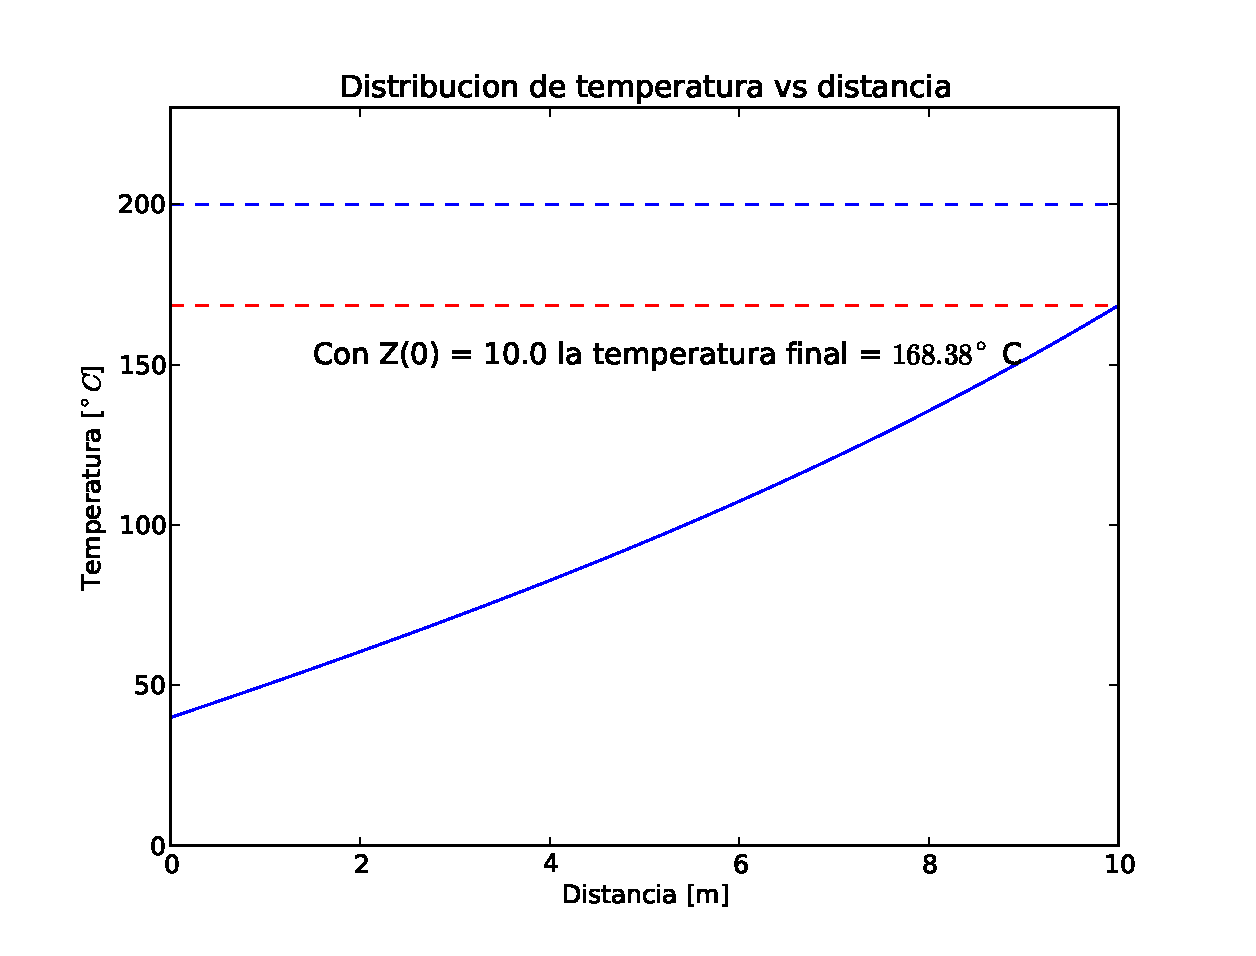
\includegraphics[scale=0.45]{MetDisparo01.eps} 
%\end{figure}
%\end{frame}
%\begin{frame}
%El resultado obtenido difiere de las condiciones de frontera $T(10)=200$, por lo que hacemos ahora otra suposición: $Z(0)=20$ y realizar de nuevo el cálculo.
%\end{frame}
%\begin{frame}
%\fontsize{12}{12}\selectfont
%\begin{center}
%\begin{tabular}{c | c | c}
%x & y[0] & y[1] \\ \hline 
%0.0000e+00 & 4.0000e+01 & 1.4000e+01 \\ \hline
%1.0000e+00 & 5.4123e+01 & 1.4270e+01 \\ \hline
%2.0000e+00 & 6.8588e+01 & 1.4684e+01 \\ \hline
%3.0000e+00 & 8.3540e+01 & 1.5244e+01 \\ \hline
%4.0000e+00 & 9.9127e+01 & 1.5957e+01 \\ \hline
%5.0000e+00 & 1.1551e+02 & 1.6829e+01 \\ \hline
%6.0000e+00 & 1.3284e+02 & 1.7870e+01 \\ \hline
%7.0000e+00 & 1.5131e+02 & 1.9090e+01 \\ \hline
%8.0000e+00 & 1.7108e+02 & 2.0500e+01 \\ \hline
%9.0000e+00 & 1.9237e+02 & 2.2116e+01 \\ \hline
%1.0000e+01 & 2.1539e+02 & 2.3954e+01
%\end{tabular}
%\end{center}
%\end{frame}
%\begin{frame}
%\frametitle{Gráficamente con $Z(0)= 14$}
%\begin{figure}
%	\centering
%	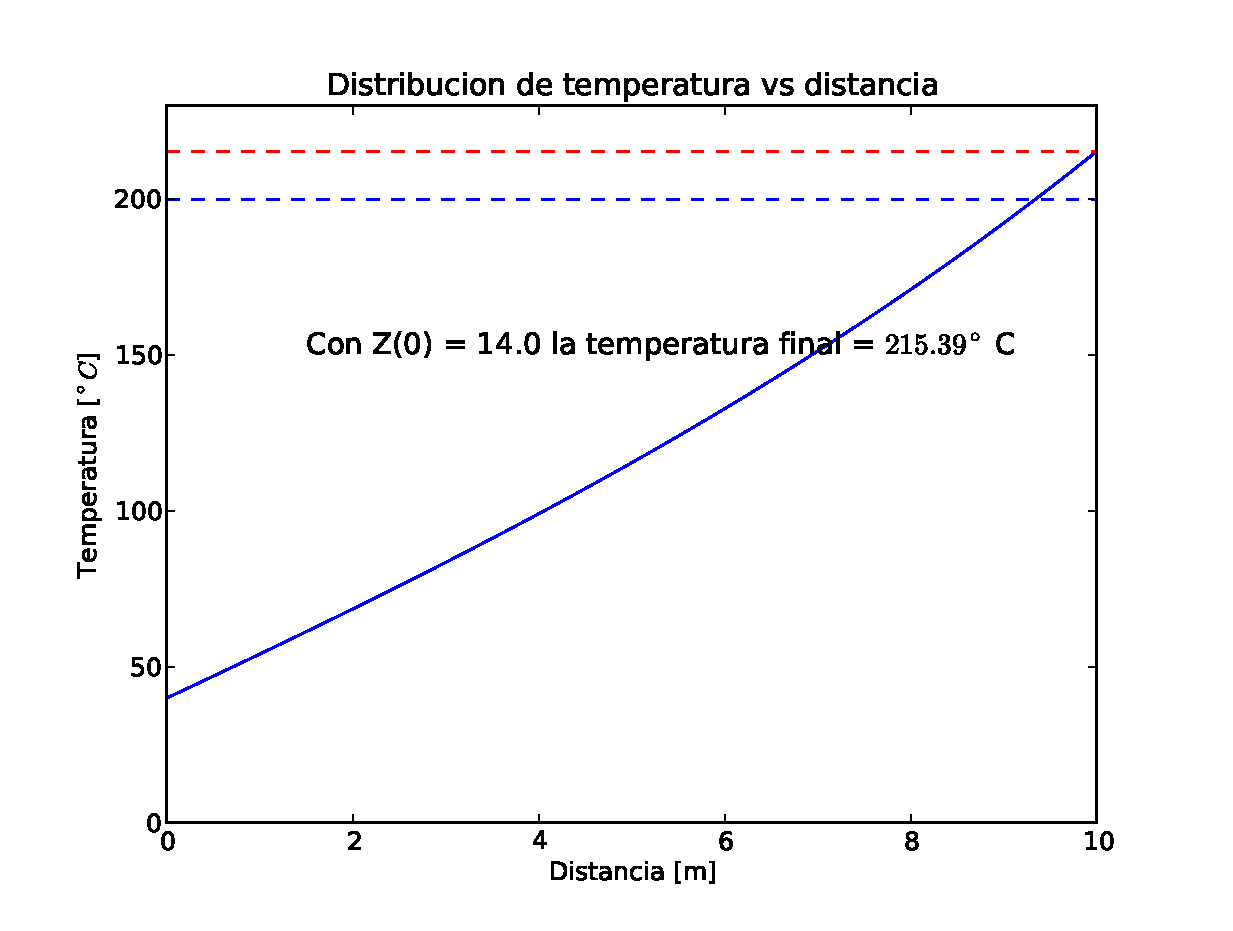
\includegraphics[scale=0.45]{MetDisparo02.eps} 
%\end{figure}
%\end{frame}
%\begin{frame}
%Ahora como la EDO original es lineal, los valores
%\[ \begin{matrix}
%Z(0) = 10 & T(10) = 168.38 \\
%Z(0) = 20 & T(10) = 215.39
%\end{matrix} \]
%están relacionados linealmente. Así, podemos usarlos para calcular el valor de $Z(0)$ que resulte para $T(10)=200$.
%\\
%\bigskip
%Podemos usar una fórmula de interpolación lineal
%\[ Z(0) =  10 + \dfrac{14-10}{215.39 - 168.37}(200-168.37) = 12.69 \]
%\end{frame}
%\begin{frame}
%\fontsize{12}{12}\selectfont
%\begin{center}
%\begin{tabular}{c | c | c}
%x & y[0] & y[1] \\ \hline 
%0.0000e+00 & 4.0000e+01 & 1.2690e+01 \\ \hline
%1.0000e+00 & 5.2811e+01 & 1.2954e+01 \\ \hline
%2.0000e+00 & 6.5951e+01 & 1.3347e+01 \\ \hline
%3.0000e+00 & 7.9550e+01 & 1.3874e+01 \\ \hline
%4.0000e+00 & 9.3746e+01 & 1.4540e+01 \\ \hline
%5.0000e+00 & 1.0868e+02 & 1.5352e+01 \\ \hline
%6.0000e+00 & 1.2450e+02 & 1.6317e+01 \\ \hline 
%7.0000e+00 & 1.4137e+02 & 1.7445e+01 \\ \hline
%8.0000e+00 & 1.5945e+02 & 1.8748e+01 \\ \hline
%9.0000e+00 & 1.7893e+02 & 2.0239e+01 \\ \hline
%1.0000e+01 & 1.9999e+02 & 2.1932e+01
%\end{tabular}
%\end{center}
%\end{frame}
%\begin{frame}
%\frametitle{Gráficamente con $Z(0)= 12.69$}
%\begin{figure}
%	\centering
%	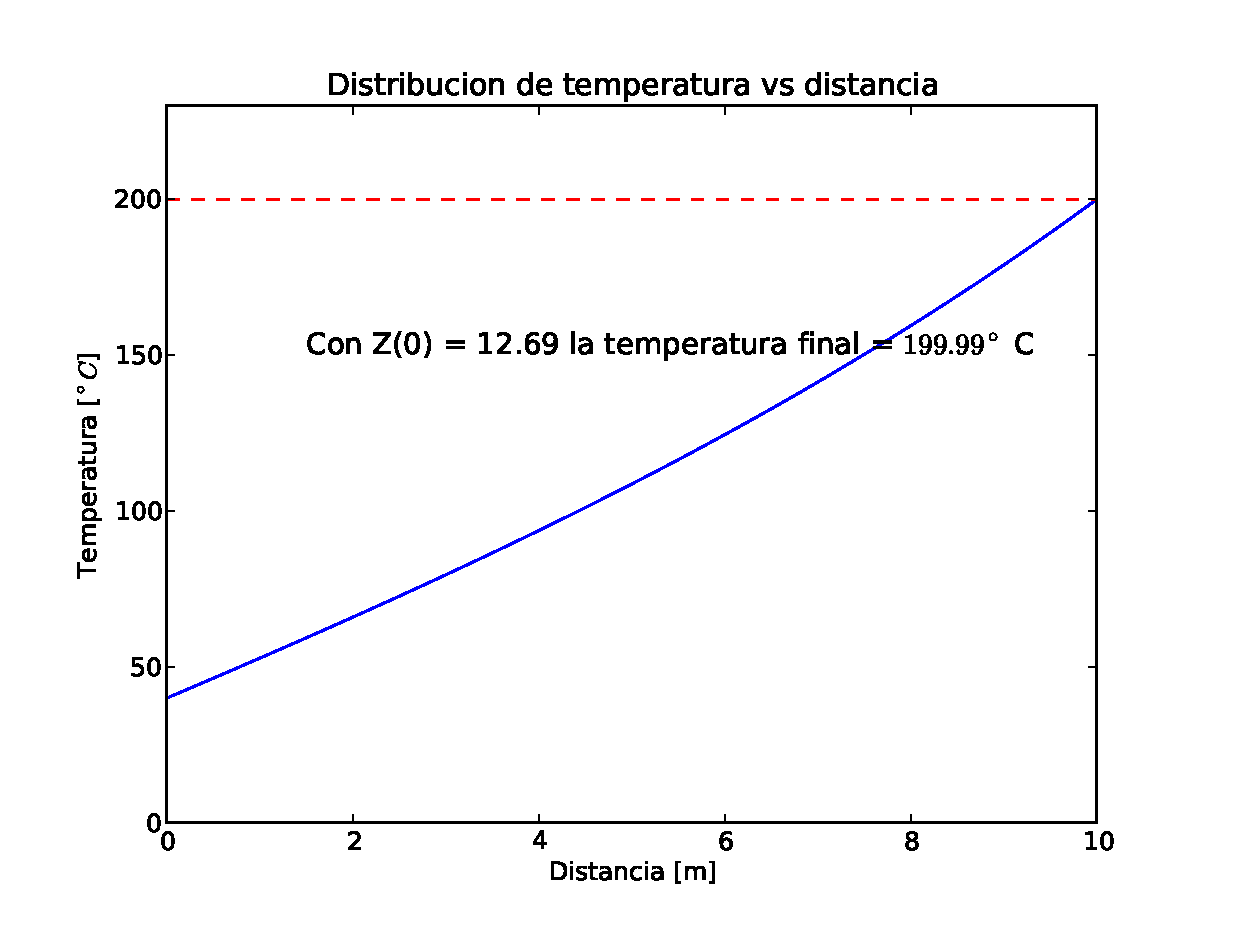
\includegraphics[scale=0.45]{MetDisparo03.eps} 
%\end{figure}
%\end{frame}
%\section{Problemas de Sturm-Liouville}
%\begin{frame}
%\frametitle{Problemas de Sturm-Liouville}
%Diversos problemas con condiciones en la frontera conducen (mediante el método de separación de variables) a la misma ecuación diferencial ordinaria
%\[ X''(x) + \lambda X(x) = 0, \hspace{1cm} (0 < x < L)\]
%con el valor propio $\lambda$, pero con distintas condiciones en los extremos:
%\begin{enumerate}
%\item $X(0) = X(L) = 0$ \hspace{1cm} Condición de Dirichlet.
%\item $X'(0) = X'(L) = 0$ \hspace{1cm} Condición de Neumann.
%\item $X(0) = X'(L) = 0$ \hspace{1cm} Condición mixta.
%\end{enumerate}
%según las condiciones de frontera.
%\end{frame}
%\begin{frame}
%Por ejemplo, en el problema de hallar la temperatura $u(x,t)$ de una varilla $0 \leq x \leq L$ con la temperatura inicial dada $u(x,0)=f(x)$.
%\\
%\bigskip
%Como problema con valores en la frontera, este problema es igual al problema de determinar la temperatura dentro de una lámina de gran tamaño que ocupe la región $0 \leq x \leq L$ en el espacio $xyz$.
%\end{frame}
%\begin{frame}
%Si su temperatura inicial sólo depende de $x$ y es independiente de $y$, $z$ (es decir, si $u(x,0)= f(x)$, entonces lo mismo será cierto de su temperatura $u=u(x,y)$ en el instante $t$. Sustituyendo
%\[u(x,t) = X(x)T(t)\]
%en la ecuación de calor
%\[ \dfrac{\partial u}{\partial t} = k \dfrac{\partial^{2} u}{\partial x^{2}}\]
%\end{frame}
%\begin{frame}
%Vemos que $X(x)$ satisface la condiciones en los extremos, si las caras $x=0$ y $x=L$ de la lámina se mantienen a temperatura cero.
%\\
%\bigskip
%Las condiciones de $X'(0) = X'(L) = 0$ si ambas caras están aisladas, y las de $X(0) = X'(L) = 0$, si una cara está aislada y la otra se mantiene a temperatura cero.
%\end{frame}
%\begin{frame}
%Pero si cada cara pierde calor hacia el medio ambiente (que se encuentra a temperatura cero) de acuerdo con la ley de enfriamiento de Newton, entonces las condiciones en los extremos asumen la forma
%\[h X(0) - X'(0) = 0 = h(X(L) + X'(L))\]
%donde $h$ es un coeficiente de transferencia de calor no negativo.
%\end{frame}
%\begin{frame}
%Al imponer diversas condiciones en los extremos sobre la solución del problema, obtenemos distintos problemas de valores propios, y por ello usamos distintos valores propios ${\lambda_{n}}$ y distintas funciones propioas $X_{n}(x)$ en la construcción de una solución formal en términos de una serie de potencias
%\[ u(x,t) = \sum c_{n} X_{n}(x) T_{n}(x)\]
%del problema con valores en la frontera. El paso final en esta construcción es la elección del coeficiente ${c_{n}}$ en la ecuación anterior de modo que
%\[u(x,0) = \sum c_{n} T_{n}(0)X_{n}(x)= f(x) \]
%\end{frame}
%\begin{frame}
%Por lo que necesitamos un desarrollo en términos de funciones propias de la función dada $f(x)$, en términos de las funciones propias del problema con valores en los extremos correspondientes.
%\end{frame}
%\begin{frame}
%\frametitle{Problemas de Sturm-Liouville}
%Para unificar y generalizar el método de separación de variables, es útil formular un tipo general de problema de valores propios que incluya como casos particulares a los ya mencionados.
%\\
%\bigskip
%La ecuación inicial, con $y$ en vez de $X$ como variable dependiente, se puede escribir como
%\[ \dfrac{d}{dx} \left[ p(x) \dfrac{dy}{dx} \right] - q(x) y + \lambda r(x) y = 0\]
%donde $p(x)=r(x) \equiv 1$ y $q(x) \equiv 0$
%\end{frame}
%\begin{frame}
%Podemos asegurar que casi cualquier ecuación diferencial lineal de segundo orden de la forma
%\[ A(x) y'' + B(x) y' + C(x) y + \lambda D(x) y = 0\]
%asume la forma indicada después de multiplicar por un factor adecuado.
%\end{frame}
%\begin{frame}
%\frametitle{Ejemplo}
%Si multiplicamos la ecuación paramétrica de Bessel de orden $n$
%\[ x^{2} y'' + xy' + (\lambda x^{2} - n^{2}) y = 0, \hspace{1cm} x>0\]
%por $1/x$, podemos escribir el resultado como
%\[ \dfrac{d}{dx} \left[ x \dfrac{dy}{dx} \right] - \dfrac{n^{2}}{x}y + \lambda x y = 0\]
%que tiene la forma S-L, con $p(x)=r(x)= x$ y $q(x) = n^{2}/x$
%\end{frame}
%\begin{frame}
%Imponiendo sobre las soluciones de la ecuación anterior, en un intervalo abierto acotado $(a,b)$ las siguientes condiciones -lineales- homogéneas en los extremos:
%\[ \begin{split}
%\alpha_{1} y(a) - \alpha_{2} y'(a) =& 0 \\
%\beta_{1} y(b) - \beta_{2} y'(b) =& 0
%\end{split} \]
%donde los coeficientes $\alpha_{1},\alpha_{2},\beta_{1},\beta_{2}$ son constantes.
%\end{frame}
%\begin{frame}
%Además de ser homogéneas, las condiciones están \textit{separadas}, en el sentido de que una de ellas implica los valores de $y(x)$ y $y'(x)$ en un extremo $x=a$, mientras que la otra implica los valores en el otro extremo $x=b$. Nótese que las condiciones $y(a)=y'(b)=0$ son d ela forma dada, con $\alpha_{1}=\beta_{2}=1$ y $\alpha_{2}=\beta_{1}=0$
%\end{frame}
%\subsection{Definición de un problema Sturm-Liouville}
%\begin{frame}
%\frametitle{Definición de un problema Sturm-Liouville}
%Un problema de Sturm-Liouville es un problema con valores en la frontera de la forma
%\[\dfrac{d}{dx} \left[ p(x) \dfrac{dy}{dx} \right] - q(x) y + \lambda r(x) y = 0, \hspace{1cm} a<x<b \]
%\[ \begin{split}
%\alpha_{1} y(a) - \alpha_{2} y'(a) =& 0 \\
%\beta_{1} y(b) - \beta_{2} y'(b) =& 0
%\end{split} \]
%donde tanto $\alpha_{1}$ y $\alpha_{2}$ como $\beta_{1}$ y $\beta_{2}$ son diferentes de cero. El parámetro $\lambda$ es el \textit{eingenvalor} cuyos posibles valores (constantes) se buscan.
%\end{frame}
%\begin{frame}
%\frametitle{Ejemplo}
%Se obtienen diferentes problemas de Sturm-Liouville complementando la ecuación diferencial
%\[ y'' + \lambda y = 0 \hspace{1cm} 0 < x < L\]
%con alguna de las diferentes condiciones de valores en la frontera homogéneas
%\begin{itemize}[<+->]
%\item $y(0) = y(L) = 0$, donde $\alpha_{1} = \beta_{1} = 1$ y $\alpha_{2} = \beta_{2} = 0$
%\item $y'(0) = y'(L) = 0$, donde $\alpha_{1} = \beta_{1} = 0$ y $\alpha_{2} = \beta_{2} = 1$
%\item $y(0) = y'(L) = 0$, donde $\alpha_{1} = \beta_{2} = 1$ y $\alpha_{2} = \beta_{1} = 0$
%\end{itemize}
%\end{frame}
%\begin{frame}
%Nótese que el problema S-L siempre tiene la solución trivial $y \equiv 0$, por consiguiente se buscan los valores de $\lambda$ (eingenvalores) para los cuales este problema tiene una solución real \textit{no trivial} (una eigenfunción) y cada eigenvalor cuenta con su eigenfunción asociada (o eigenfunciones).
%\\
%\bigskip
%Puede verse que cualquier constante (diferente de cero) múltiplo de una eigenfunción será también una eigenfunción.
%\end{frame}
%\subsection{Eigenvalores de Sturm-Liouville}
%\begin{frame}
%\frametitle{Eigenvalores de Sturm-Liouville}
%Supongamos que las funciones $p(x), p'(x),q(x)$ y $r(x)$ de la ecuación S-L son continuas en el intervalo $[a,b]$ y que tanto $p(x)>0$ como $r(x)>0$ en cada punto de $[a,b]$. De este modo los eigenvalores del problema de S-L, constituyen una sucesión creciente
%\[ \lambda_{1} < \lambda_{2} < \lambda_{3} < \ldots < \lambda_{n-1} < \lambda_{n} < \ldots\]
%de números reales, con
%\[ \lim_{n \rightarrow \infty} \lambda_{n} = + \infty\]
%Salvo por un factor constante, solo una eigenfunción $y_{n}(x)$ se asocia con cada eigenvalor $\lambda_{n}$.
%\end{frame}
%\begin{frame}
%Además, si $q(x) \geq 0$ en $[a,b]$ y los coeficientes $\alpha_{1},\alpha_{2},\beta_{1},\beta_{2}$ en la definición de S-L, son todos no negativos, entonces, los eigenvalores son todos no negativos.
%\\
%\bigskip
%Algunas veces el problema de S-L se llama \textbf{regular} si se satisface el resultado anterior, en caso contrario, es \textbf{singular}.
%\end{frame}
%\section{Una varilla delgada}
%\begin{frame}
%\frametitle{Una varilla delgada de metal}
%Sea una varilla delgada de metal con longitud $H$, sus extremos están conectados a distintas fuentes de calor:
%\begin{center}
%\begin{tikzpicture}[font=\small]
%\draw [fill=blue!20](0,0) rectangle node {$T_{L}$} (2,4);
%\draw (2,1.8) rectangle (3.5,2.2);
%\draw (4,1.8) rectangle (5.5,2.2);
%\draw [fill=blue!20] (5.5,0) rectangle node {$T_{R}$} (7.5,4);
%\draw [<->](2,1.3) -- node [midway, below] {x}(3.5,1.3);
%\draw [dashed] (3.5,2.2) -- (3.5,1.25);
%\draw [dashed] (4,2.2) -- (4,1.25);
%\draw [<-](4,1.3) -- node [midway, below] {dx}(4.6,1.3);
%\draw [<->] (2,0.1) -- node [midway, above] {H} (5.5,0.1);
%\draw (3.5,4) node {$T_{\infty}$};
%\end{tikzpicture}
%\end{center}
%\end{frame}
%\begin{frame}
%\fontsize{12}{12}\selectfont
%Si el calor sale de la superficie de la varilla únicamente por transferencia de calor, por medio de convección, la ecuación de temperatura es:
%\[ -A \dfrac{d}{dx} k(x) \dfrac{d}{dx} T(x) + h_{c} PT(x) = h_{c} PT_{\infty} + AS(x)\]
%donde
%\begin{itemize}
%\item $T(x)$ es la temperatura del punto que se encuentra a una distancia $x$ del extremo izquierdo.
%\item $A$ es el área constante de una sección transversal de la varilla.
%\item k es la conductividad térmica.
%\item P es el perímetro de la varilla.
%\item $h_{c}$ es el coeficiente de transferencia de calor por convección.
%\item $T_{\infty}$ es la temperatura neta del aire.
%\item S es la fuente de calor.
%\end{itemize}
%\end{frame}
%\begin{frame}
%Las condiciones de frontera son:
%\[ \begin{split} T(0) =& T_{L} \\
%T(H) =& T_{R}
%\end{split} \]
%Si $T^{0}$ se define como:
%\[ T^{0} = T - T_{\infty} \]
%\end{frame}
%\begin{frame}
%La ecuación de temperatura la podemos expresar como:
%\[ - \dfrac{d}{dx}k(x) \dfrac{d}{dx} T^{0}(x) + h_{c} \dfrac{P}{A} T^{0}(x) = S(x) \]
%El primer término representa la difusión del calor, el segundo es la pérdida de calor en el aire por medio de la convección y el lado derecho es la fuente de calor.
%\end{frame}
%\begin{frame}
%Otro ejemplo de una EDO con forma similar es la ecuación de difusión de neutrones dada por:
%\[ - \dfrac{d}{dx} D(x) \dfrac{d}{dx} \Psi (x) + \sum_{a} \Psi (x) = S(x) \]
%Donde $\Psi$ es el flujo de neutrones, $D$ es el coeficiente de difusión y $S$ es la fuente de neutrones.
%\\
%\bigskip
%El primer término indica la difusión de neutrones, el segundo la pérdida por absorción y el lado derecho es la fuente de neutrones.
%\end{frame}
%\begin{frame}
%Considerando en otros casos dentro de la física para problemas con difusión, si se expresa en términos de:
%\[- \dfrac{d}{dx} p(x) \dfrac{d}{dx} \phi (x) + q(x) \phi (x) = S(x)  \]
%siendo ésta, una ley de conservación de la difusión.
%\end{frame}
%\begin{frame}
%Integrando la ecuación anterior en el intervalo $[a,b]$, se obtiene que:
%\[ Z(b) - Z(a) + \int_{b}^{a} q(x) \phi (x) dx = \int_{b}^{a} S(x) dx \]
%donde
%\[ Z(x) = - p(x) \dfrac{d}{dx} \phi (x) \]
%Los términos primero y segundo de la primera ecuación aquí mostrada, son respectivamente, el flujo hacia adentro y el flujo hacia afuera de la propiedad representada por $\phi$, el tercer término es la pérdida total en $[a,b]$ y el lado derecho, es la fuente total en $[a,b]$.
%\end{frame}
%\subsection{Problemas con valores en la frontera para varillas y láminas}
%\begin{frame}
%\frametitle{Problemas con valores en la frontera para varillas y láminas}
%Consideremos una EDO de segundo orden con valores en la frontera
%\[ - \phi'' (x) + q \phi (x) = S(x), \hspace{1cm} 0< x < H \]
%con condiciones de frontera:
%\begin{itemize}
%\item $\phi'(0) = 0$, condición de frontera izquierda.
%\item $\phi'(H) = \phi'_{R}$, condición de frontera derecha
%\end{itemize}
%\end{frame}
%\begin{frame}
%Si dividimos el dominio en $N$ intervalos de igual longitud, se obtiene una retícula donde los intervalos miden $h = H/N$
%\begin{center}
%\begin{tikzpicture}[font=\small]
%\draw (0,1) node {$\phi'=0$};
%\draw (7,1) node {$\phi'=\phi_{R}$};
%\draw (-1.3,0) -- (8,0);
%\foreach \x in {-1,...,7}
%	\draw [fill=red!25](\x,0) circle (0.05);
%\draw (-1.3,-0.5) node {x=-h};
%\draw (0,-0.5) node {0};
%\draw (1,-0.5) node {h};
%\draw (2,-0.5) node {2h};
%\draw (3,-0.5) node {3h};
%\draw (7,-0.5) node {Nh=H};
%\draw (-1.3,-1) node {i=0};
%\draw (0,-1) node {1};
%\draw (1,-1) node {2};
%\draw (2,-1) node {3};
%\draw (3,-1) node {4};
%\draw (6,-1) node {N};
%\draw (7,-1) node {N=N+1};
%\end{tikzpicture}
%\end{center}
%\end{frame}
%\begin{frame}
%Usando una aproximación por diferencias centrales al primer término de la EDO de segundo orden, obtenemos la ecuación en diferencias para
%la $i$-ésima retícula:
%\[ \dfrac{(-\phi_{i-1} + 2 \phi_{i} - \phi_{i+1})}{h^{2}} + q \phi_{i} = S_{i} \]
%donde $\phi_{i}=\phi(x_{i})$, $S_{i}=S(x_{i})$ y $q$ es constante.
%\end{frame}
%\begin{frame}
%Al multiplicar por $h^{2}$
%\[ - \phi_{i-1} + (2-w) \phi_{i} - \phi_{i+1} = h^{2}S_{i} \]
%donde $w=qh^{2}$.
%\\
%\bigskip
%Esta ecuación se puede aplicar a todos los puntos de la retícula, excepto cuando $i = 1$ e $i = N+1$.
%\end{frame}
%\begin{frame}
%La condición de la frontera izquierda $\phi'(0) = 0$, es equivalente a una condición simétrica en la frontera llamada condición adiabática en la frontera en el caso de la transferencia de calor.
%\\
%\bigskip
%Si se considera un punto hipotético de la retícula $i = 0$ localizado en $x = -h$, la ecuación anterior en el caso $i = 1$ es:
%\[-\phi_{0} + (2+w)\phi_{1} - \phi_{2} = h^{2}S_{1} \]
%\end{frame}
%\begin{frame}
%En esta ecuación
%\[-\phi_{0} + (2+w)\phi_{1} - \phi_{2} = h^{2}S_{1} \]
%podemos hacer $\phi_{0} = \phi_{2}$ debido a la simetría. Dividiendo entre dos, obtenemos lo siguiente:
%\[ (1 + \dfrac{w}{2}) \phi_{1} - \phi_{2} = \dfrac{1}{2} h^{2}S_{1}\]
%como $\phi_{N+1}= \phi(H)=\phi_{R}$ en la frontera derecha, la ecuación con $i=N$ es:
%\[ -\phi_{N+1} + (2+w) \phi_{N} = h^{2}S_{N} + \phi_{R}\]
%\end{frame}
%\begin{frame}
%Ordenando los términos anteriores:
%%\fontsize{10}{10}\selectfont
%\[ \scriptsize{\begin{matrix}
%(1+\frac{w}{2})\phi_{1} & -\phi_{2}      &                &           &            & & = h^{2}\frac{S_{1}}{2} \\
%-\phi_{1}               & +(2+w)\phi_{2} & -\phi_{3}      &           &            & & = h^{2}S_{2} \\
%                        & \phi_{2}       & +(2+w)\phi_{3} & -\phi_{4} &            & & = h^{2}S_{3} \\
%                        &                &                &           &            & & \ldots \\
%                        &                &                &           &            & & \ldots \\
%                        &                &                &           &-\phi_{N+1} & +(2+w)\phi_{N} & = h^{2}S_{N}+\phi_{R} 
%\end{matrix}} \]
%\end{frame}
%\begin{frame}
%Que en forma matricial, resulta
%\fontsize{10}{10}\selectfont
%\[ \small{\begin{bmatrix}
%1+w/2 & -1 & 0 & 0 & 0 & 0 \\
%-1 & 2+w & -1 & 0 & 0 & 0 \\
%0 & -1 & 2+w & -1 & 0 & 0 \\
%0 & 0 & 0 + \ddots & -1 & 0 & 0 \\
%0 & 0 & 0 & 0 & -1 & 2+w
%\end{bmatrix} 
%\begin{bmatrix}
%\phi_{1} \\
%\phi_{2} \\
%\phi_{3} \\
%\ddots \\
%\phi_{N} \\
%\end{bmatrix} =
%\begin{bmatrix}
%h^{2}S_{1}/2 \\
%h^{2}S_{2} \\
%h^{2}S_{3} \\
%\ddots \\
%h^{2}S_{N}+\phi_{R} \\
%\end{bmatrix}}
%\]
%Todos los elementos de la matriz son cero, excepto los de las tres diagonales. Esta forma especial recibe el nombre de \emph{matriz tridiagonal}, y aparece muy a menudo en los métodos numéricos para problemas con valores en la frontera.
%\end{frame}
\end{document}